%%Introduction

In this Section, we consider models with a photon, a W boson, a Z boson or a Higgs boson in the final state, 
accompanied by Dark Matter particles that either couple directly to the boson or are mediated by 
a new particle. The experimental signature is identified as \textit{V+MET}. 

These models are interesting both as extensions of models where the gluon provides the visible object,
and as stand-alone models with final states that cannot be generated by the models in
Section~\ref{subsec:MonojetLikeModels}.

%%%Classification of models

The models considered can be divided in four categories:
\begin{description}
 \item[EFT models where the boson is radiated from the initial state]: as depicted in 
 the top diagram of Figure~\ref{fig:VPlusMET_EFT}, these  models follow the nomenclature and theory 
 for the EFT benchmarks commonly used by MET+X searches~\cite{Goodman:2010ku}. 
 \item[EFT models where the boson is directly coupled to DM]: shown in the bottom of Figure~\ref{fig:VPlusMET_EFT},
 these models 
 \item[Simplified models where the boson is radiated from the initial state]
 \item[Specific simplified models]
\end{description}

\begin{figure}[h!]
  \centering
    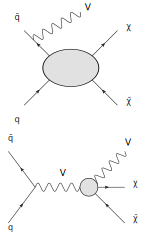
\includegraphics[width=0.5\textwidth]{figures/VPlusMET_EFT}
  \caption{Sketch of EFT models for V+MET searches, adapted from~\citep{Nelson:2013pqa}. \label{fig:VPlusMET_EFT}}
\end{figure}